% =============================================================================
% 01-intro-performance.tex — Week 1: Computer Architecture, Organization,
% and Performance Measurement
%
% Course: Computer Organization and Architecture (PCC CS-401)
% Anchor reading: Hamacher Ch. 1 (computer organization, classes of computers,
%                 performance) — chapter-level, standard treatment (Hamacher
%                 index not yet built);
%                 Patterson & Hennessy, ARM Edition, Ch. 1, Sec. 1.1 (p.3,
%                 architecture vs. organization), Sec. 1.6 (p.28, performance
%                 equation, CPI, MIPS, Amdahl's Law) — page-cited via
%                 master_supporting_docs/CS401/supporting_books/PattersonHennessy2017/index.md
%                 (built 2026-08-07).
%
% Compile with: /compile-latex CS401/01-intro-performance
% =============================================================================

\documentclass[aspectratio=169]{beamer}
% =============================================================================
% Preambles/header.tex — shared LaTeX/Beamer preamble for this project
%
% Use from a Beamer lecture by prepending:
%     % =============================================================================
% Preambles/header.tex — shared LaTeX/Beamer preamble for this project
%
% Use from a Beamer lecture by prepending:
%     % =============================================================================
% Preambles/header.tex — shared LaTeX/Beamer preamble for this project
%
% Use from a Beamer lecture by prepending:
%     \input{header}
% and compiling with TEXINPUTS=../Preambles:$TEXINPUTS (the /compile-latex
% skill does this automatically).
%
% PALETTE CONTRACT. Color names defined here MUST match the names in
% Quarto/theme-template.scss so Beamer and Quarto renderings use the same
% palette. The scripts/check-palette-sync.sh script enforces this.
%
% To customize: edit the HEX values below AND the matching $variable in
% Quarto/theme-template.scss, then run scripts/check-palette-sync.sh.
%
% TITLE PAGE. A formal, serif (Libertine) title-page template is defined in
% the Beamer-only block below (\setbeamertemplate{title page}) -- title,
% subtitle, a thin gold rule, then \author/\institute/\date. Frametitle and
% body text remain on Beamer's sans-serif default. No SCSS counterpart is
% needed for this (font/layout only, no new colors).
% =============================================================================

% -----------------------------------------------------------------------------
% Engine detection + encoding
%
% Our /compile-latex skill uses XeLaTeX, where inputenc is unnecessary and
% can produce encoding warnings. Only load inputenc under pdfTeX.
% -----------------------------------------------------------------------------
\usepackage{iftex}
\ifPDFTeX
  \usepackage[utf8]{inputenc}
\fi

\usepackage{amsmath, amssymb, amsthm}
\usepackage{booktabs}
\usepackage{graphicx}

% -----------------------------------------------------------------------------
% Serif face for the title page (formal/academic look). Linux Libertine is
% XeLaTeX- and pdfTeX-safe and redefines \rmdefault, so \rmfamily picks it up
% everywhere \rmfamily is used explicitly. Body text and frametitles stay on
% Beamer's own sans-serif default (unaffected) -- only the title-page
% \setbeamerfont{...} overrides below opt in to \rmfamily.
% -----------------------------------------------------------------------------
\usepackage{libertine}

% -----------------------------------------------------------------------------
% PALETTE — mirrors Quarto/theme-template.scss variable names.
% Load xcolor and define colors BEFORE anything that references them
% (notably hyperref, hypersetup, and the Beamer color assignments).
% -----------------------------------------------------------------------------
\usepackage{xcolor}

\definecolor{primary-blue}{HTML}{012169}      % headings, accents
\definecolor{primary-gold}{HTML}{B9975B}      % emphasis, borders
\definecolor{highlight-yellow}{HTML}{F2A900}  % markers, alerts
\definecolor{light-bg}{HTML}{E8EDF5}          % title / section backgrounds
\definecolor{jet}{HTML}{1A1A1A}               % body text

% Semantic colors (used in diagrams and annotations)
\definecolor{positive}{HTML}{15803D}          % good / observed / identified
\definecolor{negative}{HTML}{B91C1C}          % bad / problematic / bias
\definecolor{neutral}{HTML}{525252}           % reference / context

% Highlight accents (match .hi-* classes in the SCSS)
\definecolor{hi-slate}{HTML}{314F4F}
\definecolor{hi-green}{HTML}{2E8B57}
\definecolor{hi-red}{HTML}{C41E3A}

% Semantic aliases so skill templates and snippets can write
% \textcolor{accent}{...} without hard-coding "primary-blue".
\colorlet{accent}{primary-blue}
\colorlet{accent2}{primary-gold}

% -----------------------------------------------------------------------------
% Hyperref — loaded AFTER xcolor + palette so link colors resolve.
% -----------------------------------------------------------------------------
\usepackage{hyperref}
\hypersetup{colorlinks=true, linkcolor=primary-blue, urlcolor=primary-blue,
            citecolor=primary-blue, pdfborder={0 0 0}}

% -----------------------------------------------------------------------------
% Course code — set once per deck (after \input{header}, before \begin{document})
% via \coursecode{CS401}. Shown in the footer on every slide so a deck's course
% is identifiable without opening the title page. Empty by default.
% -----------------------------------------------------------------------------
\makeatletter
\newcommand{\coursecode}[1]{\gdef\@coursecodetext{#1}}
\gdef\@coursecodetext{}
\makeatother

% -----------------------------------------------------------------------------
% Beamer theme assignments (only apply under Beamer).
%
% We detect Beamer via \@ifclassloaded{beamer}, which is the documented,
% non-internal way. This must be wrapped in \makeatletter/\makeatother
% because \@ifclassloaded contains an @-catcode character.
% -----------------------------------------------------------------------------
\makeatletter
\@ifclassloaded{beamer}{%
  \usefonttheme{professionalfonts}
  \setbeamercolor{structure}{fg=primary-blue}
  \setbeamercolor{frametitle}{fg=primary-blue}
  \setbeamercolor{title}{fg=primary-blue}
  \setbeamercolor{subtitle}{fg=primary-gold}
  \setbeamercolor{author}{fg=primary-blue}
  \setbeamercolor{institute}{fg=neutral}
  \setbeamercolor{date}{fg=primary-gold}
  \setbeamercolor{itemize item}{fg=primary-blue}
  \setbeamercolor{itemize subitem}{fg=primary-gold}
  \setbeamercolor{alerted text}{fg=primary-gold}
  \setbeamercolor{block title}{fg=white, bg=primary-blue}
  \setbeamercolor{block body}{bg=light-bg}
  % Semantic block variants: block=definition/concept (blue), exampleblock=
  % worked example (green/positive), alertblock=key takeaway or caution (gold).
  % Keep to <=2 colored boxes per slide across ALL three variants (INV-7).
  \setbeamercolor{block title example}{fg=white, bg=positive}
  \setbeamercolor{block body example}{bg=light-bg}
  \setbeamercolor{block title alerted}{fg=white, bg=primary-gold}
  \setbeamercolor{block body alerted}{bg=light-bg}

  % ---------------------------------------------------------------------------
  % Formal title page: serif (Libertine, via \rmfamily) for title-page
  % elements only. Body text, itemize, and frametitle are intentionally left
  % on Beamer's sans-serif default -- \usebeamerfont{title} is also what
  % \transitionslide (below) uses for its big centered text, so section
  % transitions pick up the same serif treatment for free.
  % ---------------------------------------------------------------------------
  \setbeamerfont{title}{family=\rmfamily, series=\bfseries, size=\Large}
  \setbeamerfont{subtitle}{family=\rmfamily, shape=\itshape, size=\normalsize}
  \setbeamerfont{author}{family=\rmfamily, size=\normalsize}
  \setbeamerfont{institute}{family=\rmfamily, size=\scriptsize}
  \setbeamerfont{date}{family=\rmfamily, size=\scriptsize}

  \setbeamertemplate{title page}{
    \vfill
    \begin{center}
      {\usebeamerfont{title}\usebeamercolor[fg]{title}\inserttitle\par}
      \vspace{0.15cm}
      {\usebeamerfont{subtitle}\usebeamercolor[fg]{subtitle}\insertsubtitle\par}
      \vspace{0.45cm}
      {\color{primary-gold}\rule{0.42\textwidth}{0.6pt}\par}
      \vspace{0.45cm}
      {\usebeamerfont{author}\usebeamercolor[fg]{author}\insertauthor\par}
      \vspace{0.35cm}
      {\usebeamerfont{institute}\usebeamercolor[fg]{institute}\insertinstitute\par}
      \vspace{0.35cm}
      {\usebeamerfont{date}\usebeamercolor[fg]{date}\insertdate\par}
    \end{center}
    \vfill
  }

  % Minimal footer: course code (left) + page X / N (right), no navigation clutter
  \setbeamertemplate{navigation symbols}{}
  \setbeamertemplate{footline}{%
    \color{neutral}\footnotesize\hspace{0.7em}\@coursecodetext\hfill
    \insertframenumber/\inserttotalframenumber\hspace{0.7em}\vspace{0.3em}}
}{}
\makeatother

% -----------------------------------------------------------------------------
% TikZ setup — libraries the snippet gallery uses
% -----------------------------------------------------------------------------
\usepackage{tikz}
\usetikzlibrary{arrows.meta, positioning, calc, decorations.pathreplacing,
                fit, shapes.geometric, backgrounds}

% Shared TikZ styles — snippets and hand-written diagrams can pick these up
% via `\begin{tikzpicture}[every node/.style={...}]` or by naming specific
% styles (e.g., `\node[dag-node] (X) at (0,0) {X};`).
\tikzset{
  % Node styles for causal DAGs and similar
  dag-node/.style = {
    draw=primary-blue, fill=light-bg, rounded corners=2pt,
    minimum width=1.2cm, minimum height=0.9cm, align=center, font=\small
  },
  decision-node/.style = {
    draw=primary-gold, fill=white, diamond, aspect=1.8,
    minimum width=1.8cm, minimum height=1.2cm, align=center, font=\small,
    inner sep=1pt
  },
  % Edge styles — observed vs counterfactual
  observed-edge/.style = {-{Latex[length=2.5mm]}, thick, draw=jet},
  counterfactual-edge/.style = {-{Latex[length=2.5mm]}, thick, draw=neutral, dashed},
  confound-edge/.style = {-{Latex[length=2.5mm]}, thick, draw=negative, dashed},
  % Data-point styles for plots
  observed-dot/.style = {fill=primary-blue, draw=primary-blue, circle, inner sep=1.2pt},
  counterfactual-dot/.style = {fill=white, draw=neutral, circle, inner sep=1.2pt}
}

% -----------------------------------------------------------------------------
% Convenience macros
% -----------------------------------------------------------------------------
\newcommand{\muted}[1]{\textcolor{neutral}{#1}}
\newcommand{\key}[1]{\textcolor{primary-gold}{\textbf{#1}}}
\newcommand{\good}[1]{\textcolor{positive}{#1}}
\newcommand{\bad}[1]{\textcolor{negative}{#1}}

% Standout frame macro: full-bleed dark background for section transitions.
% Beamer-only (uses \begin{frame}/\setbeamercolor/\usebeamerfont) -- do not
% call from an article-class file (e.g. Notes/<CODE>/*-notes.tex). \muted,
% \key, \good, \bad, and \coursecode above are plain xcolor/gdef and are
% safe to use from either class; verified when Notes/article-class support
% was added.
% Expand: \transitionslide{Your transition title}
\newcommand{\transitionslide}[1]{%
  \begingroup
  \setbeamercolor{background canvas}{bg=primary-blue}
  \begin{frame}[plain]
    \centering
    \vfill
    {\usebeamerfont{title}\color{white}\Large #1\par}
    \vfill
  \end{frame}
  \endgroup
}

% and compiling with TEXINPUTS=../Preambles:$TEXINPUTS (the /compile-latex
% skill does this automatically).
%
% PALETTE CONTRACT. Color names defined here MUST match the names in
% Quarto/theme-template.scss so Beamer and Quarto renderings use the same
% palette. The scripts/check-palette-sync.sh script enforces this.
%
% To customize: edit the HEX values below AND the matching $variable in
% Quarto/theme-template.scss, then run scripts/check-palette-sync.sh.
%
% TITLE PAGE. A formal, serif (Libertine) title-page template is defined in
% the Beamer-only block below (\setbeamertemplate{title page}) -- title,
% subtitle, a thin gold rule, then \author/\institute/\date. Frametitle and
% body text remain on Beamer's sans-serif default. No SCSS counterpart is
% needed for this (font/layout only, no new colors).
% =============================================================================

% -----------------------------------------------------------------------------
% Engine detection + encoding
%
% Our /compile-latex skill uses XeLaTeX, where inputenc is unnecessary and
% can produce encoding warnings. Only load inputenc under pdfTeX.
% -----------------------------------------------------------------------------
\usepackage{iftex}
\ifPDFTeX
  \usepackage[utf8]{inputenc}
\fi

\usepackage{amsmath, amssymb, amsthm}
\usepackage{booktabs}
\usepackage{graphicx}

% -----------------------------------------------------------------------------
% Serif face for the title page (formal/academic look). Linux Libertine is
% XeLaTeX- and pdfTeX-safe and redefines \rmdefault, so \rmfamily picks it up
% everywhere \rmfamily is used explicitly. Body text and frametitles stay on
% Beamer's own sans-serif default (unaffected) -- only the title-page
% \setbeamerfont{...} overrides below opt in to \rmfamily.
% -----------------------------------------------------------------------------
\usepackage{libertine}

% -----------------------------------------------------------------------------
% PALETTE — mirrors Quarto/theme-template.scss variable names.
% Load xcolor and define colors BEFORE anything that references them
% (notably hyperref, hypersetup, and the Beamer color assignments).
% -----------------------------------------------------------------------------
\usepackage{xcolor}

\definecolor{primary-blue}{HTML}{012169}      % headings, accents
\definecolor{primary-gold}{HTML}{B9975B}      % emphasis, borders
\definecolor{highlight-yellow}{HTML}{F2A900}  % markers, alerts
\definecolor{light-bg}{HTML}{E8EDF5}          % title / section backgrounds
\definecolor{jet}{HTML}{1A1A1A}               % body text

% Semantic colors (used in diagrams and annotations)
\definecolor{positive}{HTML}{15803D}          % good / observed / identified
\definecolor{negative}{HTML}{B91C1C}          % bad / problematic / bias
\definecolor{neutral}{HTML}{525252}           % reference / context

% Highlight accents (match .hi-* classes in the SCSS)
\definecolor{hi-slate}{HTML}{314F4F}
\definecolor{hi-green}{HTML}{2E8B57}
\definecolor{hi-red}{HTML}{C41E3A}

% Semantic aliases so skill templates and snippets can write
% \textcolor{accent}{...} without hard-coding "primary-blue".
\colorlet{accent}{primary-blue}
\colorlet{accent2}{primary-gold}

% -----------------------------------------------------------------------------
% Hyperref — loaded AFTER xcolor + palette so link colors resolve.
% -----------------------------------------------------------------------------
\usepackage{hyperref}
\hypersetup{colorlinks=true, linkcolor=primary-blue, urlcolor=primary-blue,
            citecolor=primary-blue, pdfborder={0 0 0}}

% -----------------------------------------------------------------------------
% Course code — set once per deck (after % =============================================================================
% Preambles/header.tex — shared LaTeX/Beamer preamble for this project
%
% Use from a Beamer lecture by prepending:
%     \input{header}
% and compiling with TEXINPUTS=../Preambles:$TEXINPUTS (the /compile-latex
% skill does this automatically).
%
% PALETTE CONTRACT. Color names defined here MUST match the names in
% Quarto/theme-template.scss so Beamer and Quarto renderings use the same
% palette. The scripts/check-palette-sync.sh script enforces this.
%
% To customize: edit the HEX values below AND the matching $variable in
% Quarto/theme-template.scss, then run scripts/check-palette-sync.sh.
%
% TITLE PAGE. A formal, serif (Libertine) title-page template is defined in
% the Beamer-only block below (\setbeamertemplate{title page}) -- title,
% subtitle, a thin gold rule, then \author/\institute/\date. Frametitle and
% body text remain on Beamer's sans-serif default. No SCSS counterpart is
% needed for this (font/layout only, no new colors).
% =============================================================================

% -----------------------------------------------------------------------------
% Engine detection + encoding
%
% Our /compile-latex skill uses XeLaTeX, where inputenc is unnecessary and
% can produce encoding warnings. Only load inputenc under pdfTeX.
% -----------------------------------------------------------------------------
\usepackage{iftex}
\ifPDFTeX
  \usepackage[utf8]{inputenc}
\fi

\usepackage{amsmath, amssymb, amsthm}
\usepackage{booktabs}
\usepackage{graphicx}

% -----------------------------------------------------------------------------
% Serif face for the title page (formal/academic look). Linux Libertine is
% XeLaTeX- and pdfTeX-safe and redefines \rmdefault, so \rmfamily picks it up
% everywhere \rmfamily is used explicitly. Body text and frametitles stay on
% Beamer's own sans-serif default (unaffected) -- only the title-page
% \setbeamerfont{...} overrides below opt in to \rmfamily.
% -----------------------------------------------------------------------------
\usepackage{libertine}

% -----------------------------------------------------------------------------
% PALETTE — mirrors Quarto/theme-template.scss variable names.
% Load xcolor and define colors BEFORE anything that references them
% (notably hyperref, hypersetup, and the Beamer color assignments).
% -----------------------------------------------------------------------------
\usepackage{xcolor}

\definecolor{primary-blue}{HTML}{012169}      % headings, accents
\definecolor{primary-gold}{HTML}{B9975B}      % emphasis, borders
\definecolor{highlight-yellow}{HTML}{F2A900}  % markers, alerts
\definecolor{light-bg}{HTML}{E8EDF5}          % title / section backgrounds
\definecolor{jet}{HTML}{1A1A1A}               % body text

% Semantic colors (used in diagrams and annotations)
\definecolor{positive}{HTML}{15803D}          % good / observed / identified
\definecolor{negative}{HTML}{B91C1C}          % bad / problematic / bias
\definecolor{neutral}{HTML}{525252}           % reference / context

% Highlight accents (match .hi-* classes in the SCSS)
\definecolor{hi-slate}{HTML}{314F4F}
\definecolor{hi-green}{HTML}{2E8B57}
\definecolor{hi-red}{HTML}{C41E3A}

% Semantic aliases so skill templates and snippets can write
% \textcolor{accent}{...} without hard-coding "primary-blue".
\colorlet{accent}{primary-blue}
\colorlet{accent2}{primary-gold}

% -----------------------------------------------------------------------------
% Hyperref — loaded AFTER xcolor + palette so link colors resolve.
% -----------------------------------------------------------------------------
\usepackage{hyperref}
\hypersetup{colorlinks=true, linkcolor=primary-blue, urlcolor=primary-blue,
            citecolor=primary-blue, pdfborder={0 0 0}}

% -----------------------------------------------------------------------------
% Course code — set once per deck (after \input{header}, before \begin{document})
% via \coursecode{CS401}. Shown in the footer on every slide so a deck's course
% is identifiable without opening the title page. Empty by default.
% -----------------------------------------------------------------------------
\makeatletter
\newcommand{\coursecode}[1]{\gdef\@coursecodetext{#1}}
\gdef\@coursecodetext{}
\makeatother

% -----------------------------------------------------------------------------
% Beamer theme assignments (only apply under Beamer).
%
% We detect Beamer via \@ifclassloaded{beamer}, which is the documented,
% non-internal way. This must be wrapped in \makeatletter/\makeatother
% because \@ifclassloaded contains an @-catcode character.
% -----------------------------------------------------------------------------
\makeatletter
\@ifclassloaded{beamer}{%
  \usefonttheme{professionalfonts}
  \setbeamercolor{structure}{fg=primary-blue}
  \setbeamercolor{frametitle}{fg=primary-blue}
  \setbeamercolor{title}{fg=primary-blue}
  \setbeamercolor{subtitle}{fg=primary-gold}
  \setbeamercolor{author}{fg=primary-blue}
  \setbeamercolor{institute}{fg=neutral}
  \setbeamercolor{date}{fg=primary-gold}
  \setbeamercolor{itemize item}{fg=primary-blue}
  \setbeamercolor{itemize subitem}{fg=primary-gold}
  \setbeamercolor{alerted text}{fg=primary-gold}
  \setbeamercolor{block title}{fg=white, bg=primary-blue}
  \setbeamercolor{block body}{bg=light-bg}
  % Semantic block variants: block=definition/concept (blue), exampleblock=
  % worked example (green/positive), alertblock=key takeaway or caution (gold).
  % Keep to <=2 colored boxes per slide across ALL three variants (INV-7).
  \setbeamercolor{block title example}{fg=white, bg=positive}
  \setbeamercolor{block body example}{bg=light-bg}
  \setbeamercolor{block title alerted}{fg=white, bg=primary-gold}
  \setbeamercolor{block body alerted}{bg=light-bg}

  % ---------------------------------------------------------------------------
  % Formal title page: serif (Libertine, via \rmfamily) for title-page
  % elements only. Body text, itemize, and frametitle are intentionally left
  % on Beamer's sans-serif default -- \usebeamerfont{title} is also what
  % \transitionslide (below) uses for its big centered text, so section
  % transitions pick up the same serif treatment for free.
  % ---------------------------------------------------------------------------
  \setbeamerfont{title}{family=\rmfamily, series=\bfseries, size=\Large}
  \setbeamerfont{subtitle}{family=\rmfamily, shape=\itshape, size=\normalsize}
  \setbeamerfont{author}{family=\rmfamily, size=\normalsize}
  \setbeamerfont{institute}{family=\rmfamily, size=\scriptsize}
  \setbeamerfont{date}{family=\rmfamily, size=\scriptsize}

  \setbeamertemplate{title page}{
    \vfill
    \begin{center}
      {\usebeamerfont{title}\usebeamercolor[fg]{title}\inserttitle\par}
      \vspace{0.15cm}
      {\usebeamerfont{subtitle}\usebeamercolor[fg]{subtitle}\insertsubtitle\par}
      \vspace{0.45cm}
      {\color{primary-gold}\rule{0.42\textwidth}{0.6pt}\par}
      \vspace{0.45cm}
      {\usebeamerfont{author}\usebeamercolor[fg]{author}\insertauthor\par}
      \vspace{0.35cm}
      {\usebeamerfont{institute}\usebeamercolor[fg]{institute}\insertinstitute\par}
      \vspace{0.35cm}
      {\usebeamerfont{date}\usebeamercolor[fg]{date}\insertdate\par}
    \end{center}
    \vfill
  }

  % Minimal footer: course code (left) + page X / N (right), no navigation clutter
  \setbeamertemplate{navigation symbols}{}
  \setbeamertemplate{footline}{%
    \color{neutral}\footnotesize\hspace{0.7em}\@coursecodetext\hfill
    \insertframenumber/\inserttotalframenumber\hspace{0.7em}\vspace{0.3em}}
}{}
\makeatother

% -----------------------------------------------------------------------------
% TikZ setup — libraries the snippet gallery uses
% -----------------------------------------------------------------------------
\usepackage{tikz}
\usetikzlibrary{arrows.meta, positioning, calc, decorations.pathreplacing,
                fit, shapes.geometric, backgrounds}

% Shared TikZ styles — snippets and hand-written diagrams can pick these up
% via `\begin{tikzpicture}[every node/.style={...}]` or by naming specific
% styles (e.g., `\node[dag-node] (X) at (0,0) {X};`).
\tikzset{
  % Node styles for causal DAGs and similar
  dag-node/.style = {
    draw=primary-blue, fill=light-bg, rounded corners=2pt,
    minimum width=1.2cm, minimum height=0.9cm, align=center, font=\small
  },
  decision-node/.style = {
    draw=primary-gold, fill=white, diamond, aspect=1.8,
    minimum width=1.8cm, minimum height=1.2cm, align=center, font=\small,
    inner sep=1pt
  },
  % Edge styles — observed vs counterfactual
  observed-edge/.style = {-{Latex[length=2.5mm]}, thick, draw=jet},
  counterfactual-edge/.style = {-{Latex[length=2.5mm]}, thick, draw=neutral, dashed},
  confound-edge/.style = {-{Latex[length=2.5mm]}, thick, draw=negative, dashed},
  % Data-point styles for plots
  observed-dot/.style = {fill=primary-blue, draw=primary-blue, circle, inner sep=1.2pt},
  counterfactual-dot/.style = {fill=white, draw=neutral, circle, inner sep=1.2pt}
}

% -----------------------------------------------------------------------------
% Convenience macros
% -----------------------------------------------------------------------------
\newcommand{\muted}[1]{\textcolor{neutral}{#1}}
\newcommand{\key}[1]{\textcolor{primary-gold}{\textbf{#1}}}
\newcommand{\good}[1]{\textcolor{positive}{#1}}
\newcommand{\bad}[1]{\textcolor{negative}{#1}}

% Standout frame macro: full-bleed dark background for section transitions.
% Beamer-only (uses \begin{frame}/\setbeamercolor/\usebeamerfont) -- do not
% call from an article-class file (e.g. Notes/<CODE>/*-notes.tex). \muted,
% \key, \good, \bad, and \coursecode above are plain xcolor/gdef and are
% safe to use from either class; verified when Notes/article-class support
% was added.
% Expand: \transitionslide{Your transition title}
\newcommand{\transitionslide}[1]{%
  \begingroup
  \setbeamercolor{background canvas}{bg=primary-blue}
  \begin{frame}[plain]
    \centering
    \vfill
    {\usebeamerfont{title}\color{white}\Large #1\par}
    \vfill
  \end{frame}
  \endgroup
}
, before \begin{document})
% via \coursecode{CS401}. Shown in the footer on every slide so a deck's course
% is identifiable without opening the title page. Empty by default.
% -----------------------------------------------------------------------------
\makeatletter
\newcommand{\coursecode}[1]{\gdef\@coursecodetext{#1}}
\gdef\@coursecodetext{}
\makeatother

% -----------------------------------------------------------------------------
% Beamer theme assignments (only apply under Beamer).
%
% We detect Beamer via \@ifclassloaded{beamer}, which is the documented,
% non-internal way. This must be wrapped in \makeatletter/\makeatother
% because \@ifclassloaded contains an @-catcode character.
% -----------------------------------------------------------------------------
\makeatletter
\@ifclassloaded{beamer}{%
  \usefonttheme{professionalfonts}
  \setbeamercolor{structure}{fg=primary-blue}
  \setbeamercolor{frametitle}{fg=primary-blue}
  \setbeamercolor{title}{fg=primary-blue}
  \setbeamercolor{subtitle}{fg=primary-gold}
  \setbeamercolor{author}{fg=primary-blue}
  \setbeamercolor{institute}{fg=neutral}
  \setbeamercolor{date}{fg=primary-gold}
  \setbeamercolor{itemize item}{fg=primary-blue}
  \setbeamercolor{itemize subitem}{fg=primary-gold}
  \setbeamercolor{alerted text}{fg=primary-gold}
  \setbeamercolor{block title}{fg=white, bg=primary-blue}
  \setbeamercolor{block body}{bg=light-bg}
  % Semantic block variants: block=definition/concept (blue), exampleblock=
  % worked example (green/positive), alertblock=key takeaway or caution (gold).
  % Keep to <=2 colored boxes per slide across ALL three variants (INV-7).
  \setbeamercolor{block title example}{fg=white, bg=positive}
  \setbeamercolor{block body example}{bg=light-bg}
  \setbeamercolor{block title alerted}{fg=white, bg=primary-gold}
  \setbeamercolor{block body alerted}{bg=light-bg}

  % ---------------------------------------------------------------------------
  % Formal title page: serif (Libertine, via \rmfamily) for title-page
  % elements only. Body text, itemize, and frametitle are intentionally left
  % on Beamer's sans-serif default -- \usebeamerfont{title} is also what
  % \transitionslide (below) uses for its big centered text, so section
  % transitions pick up the same serif treatment for free.
  % ---------------------------------------------------------------------------
  \setbeamerfont{title}{family=\rmfamily, series=\bfseries, size=\Large}
  \setbeamerfont{subtitle}{family=\rmfamily, shape=\itshape, size=\normalsize}
  \setbeamerfont{author}{family=\rmfamily, size=\normalsize}
  \setbeamerfont{institute}{family=\rmfamily, size=\scriptsize}
  \setbeamerfont{date}{family=\rmfamily, size=\scriptsize}

  \setbeamertemplate{title page}{
    \vfill
    \begin{center}
      {\usebeamerfont{title}\usebeamercolor[fg]{title}\inserttitle\par}
      \vspace{0.15cm}
      {\usebeamerfont{subtitle}\usebeamercolor[fg]{subtitle}\insertsubtitle\par}
      \vspace{0.45cm}
      {\color{primary-gold}\rule{0.42\textwidth}{0.6pt}\par}
      \vspace{0.45cm}
      {\usebeamerfont{author}\usebeamercolor[fg]{author}\insertauthor\par}
      \vspace{0.35cm}
      {\usebeamerfont{institute}\usebeamercolor[fg]{institute}\insertinstitute\par}
      \vspace{0.35cm}
      {\usebeamerfont{date}\usebeamercolor[fg]{date}\insertdate\par}
    \end{center}
    \vfill
  }

  % Minimal footer: course code (left) + page X / N (right), no navigation clutter
  \setbeamertemplate{navigation symbols}{}
  \setbeamertemplate{footline}{%
    \color{neutral}\footnotesize\hspace{0.7em}\@coursecodetext\hfill
    \insertframenumber/\inserttotalframenumber\hspace{0.7em}\vspace{0.3em}}
}{}
\makeatother

% -----------------------------------------------------------------------------
% TikZ setup — libraries the snippet gallery uses
% -----------------------------------------------------------------------------
\usepackage{tikz}
\usetikzlibrary{arrows.meta, positioning, calc, decorations.pathreplacing,
                fit, shapes.geometric, backgrounds}

% Shared TikZ styles — snippets and hand-written diagrams can pick these up
% via `\begin{tikzpicture}[every node/.style={...}]` or by naming specific
% styles (e.g., `\node[dag-node] (X) at (0,0) {X};`).
\tikzset{
  % Node styles for causal DAGs and similar
  dag-node/.style = {
    draw=primary-blue, fill=light-bg, rounded corners=2pt,
    minimum width=1.2cm, minimum height=0.9cm, align=center, font=\small
  },
  decision-node/.style = {
    draw=primary-gold, fill=white, diamond, aspect=1.8,
    minimum width=1.8cm, minimum height=1.2cm, align=center, font=\small,
    inner sep=1pt
  },
  % Edge styles — observed vs counterfactual
  observed-edge/.style = {-{Latex[length=2.5mm]}, thick, draw=jet},
  counterfactual-edge/.style = {-{Latex[length=2.5mm]}, thick, draw=neutral, dashed},
  confound-edge/.style = {-{Latex[length=2.5mm]}, thick, draw=negative, dashed},
  % Data-point styles for plots
  observed-dot/.style = {fill=primary-blue, draw=primary-blue, circle, inner sep=1.2pt},
  counterfactual-dot/.style = {fill=white, draw=neutral, circle, inner sep=1.2pt}
}

% -----------------------------------------------------------------------------
% Convenience macros
% -----------------------------------------------------------------------------
\newcommand{\muted}[1]{\textcolor{neutral}{#1}}
\newcommand{\key}[1]{\textcolor{primary-gold}{\textbf{#1}}}
\newcommand{\good}[1]{\textcolor{positive}{#1}}
\newcommand{\bad}[1]{\textcolor{negative}{#1}}

% Standout frame macro: full-bleed dark background for section transitions.
% Beamer-only (uses \begin{frame}/\setbeamercolor/\usebeamerfont) -- do not
% call from an article-class file (e.g. Notes/<CODE>/*-notes.tex). \muted,
% \key, \good, \bad, and \coursecode above are plain xcolor/gdef and are
% safe to use from either class; verified when Notes/article-class support
% was added.
% Expand: \transitionslide{Your transition title}
\newcommand{\transitionslide}[1]{%
  \begingroup
  \setbeamercolor{background canvas}{bg=primary-blue}
  \begin{frame}[plain]
    \centering
    \vfill
    {\usebeamerfont{title}\color{white}\Large #1\par}
    \vfill
  \end{frame}
  \endgroup
}

% and compiling with TEXINPUTS=../Preambles:$TEXINPUTS (the /compile-latex
% skill does this automatically).
%
% PALETTE CONTRACT. Color names defined here MUST match the names in
% Quarto/theme-template.scss so Beamer and Quarto renderings use the same
% palette. The scripts/check-palette-sync.sh script enforces this.
%
% To customize: edit the HEX values below AND the matching $variable in
% Quarto/theme-template.scss, then run scripts/check-palette-sync.sh.
%
% TITLE PAGE. A formal, serif (Libertine) title-page template is defined in
% the Beamer-only block below (\setbeamertemplate{title page}) -- title,
% subtitle, a thin gold rule, then \author/\institute/\date. Frametitle and
% body text remain on Beamer's sans-serif default. No SCSS counterpart is
% needed for this (font/layout only, no new colors).
% =============================================================================

% -----------------------------------------------------------------------------
% Engine detection + encoding
%
% Our /compile-latex skill uses XeLaTeX, where inputenc is unnecessary and
% can produce encoding warnings. Only load inputenc under pdfTeX.
% -----------------------------------------------------------------------------
\usepackage{iftex}
\ifPDFTeX
  \usepackage[utf8]{inputenc}
\fi

\usepackage{amsmath, amssymb, amsthm}
\usepackage{booktabs}
\usepackage{graphicx}

% -----------------------------------------------------------------------------
% Serif face for the title page (formal/academic look). Linux Libertine is
% XeLaTeX- and pdfTeX-safe and redefines \rmdefault, so \rmfamily picks it up
% everywhere \rmfamily is used explicitly. Body text and frametitles stay on
% Beamer's own sans-serif default (unaffected) -- only the title-page
% \setbeamerfont{...} overrides below opt in to \rmfamily.
% -----------------------------------------------------------------------------
\usepackage{libertine}

% -----------------------------------------------------------------------------
% PALETTE — mirrors Quarto/theme-template.scss variable names.
% Load xcolor and define colors BEFORE anything that references them
% (notably hyperref, hypersetup, and the Beamer color assignments).
% -----------------------------------------------------------------------------
\usepackage{xcolor}

\definecolor{primary-blue}{HTML}{012169}      % headings, accents
\definecolor{primary-gold}{HTML}{B9975B}      % emphasis, borders
\definecolor{highlight-yellow}{HTML}{F2A900}  % markers, alerts
\definecolor{light-bg}{HTML}{E8EDF5}          % title / section backgrounds
\definecolor{jet}{HTML}{1A1A1A}               % body text

% Semantic colors (used in diagrams and annotations)
\definecolor{positive}{HTML}{15803D}          % good / observed / identified
\definecolor{negative}{HTML}{B91C1C}          % bad / problematic / bias
\definecolor{neutral}{HTML}{525252}           % reference / context

% Highlight accents (match .hi-* classes in the SCSS)
\definecolor{hi-slate}{HTML}{314F4F}
\definecolor{hi-green}{HTML}{2E8B57}
\definecolor{hi-red}{HTML}{C41E3A}

% Semantic aliases so skill templates and snippets can write
% \textcolor{accent}{...} without hard-coding "primary-blue".
\colorlet{accent}{primary-blue}
\colorlet{accent2}{primary-gold}

% -----------------------------------------------------------------------------
% Hyperref — loaded AFTER xcolor + palette so link colors resolve.
% -----------------------------------------------------------------------------
\usepackage{hyperref}
\hypersetup{colorlinks=true, linkcolor=primary-blue, urlcolor=primary-blue,
            citecolor=primary-blue, pdfborder={0 0 0}}

% -----------------------------------------------------------------------------
% Course code — set once per deck (after % =============================================================================
% Preambles/header.tex — shared LaTeX/Beamer preamble for this project
%
% Use from a Beamer lecture by prepending:
%     % =============================================================================
% Preambles/header.tex — shared LaTeX/Beamer preamble for this project
%
% Use from a Beamer lecture by prepending:
%     \input{header}
% and compiling with TEXINPUTS=../Preambles:$TEXINPUTS (the /compile-latex
% skill does this automatically).
%
% PALETTE CONTRACT. Color names defined here MUST match the names in
% Quarto/theme-template.scss so Beamer and Quarto renderings use the same
% palette. The scripts/check-palette-sync.sh script enforces this.
%
% To customize: edit the HEX values below AND the matching $variable in
% Quarto/theme-template.scss, then run scripts/check-palette-sync.sh.
%
% TITLE PAGE. A formal, serif (Libertine) title-page template is defined in
% the Beamer-only block below (\setbeamertemplate{title page}) -- title,
% subtitle, a thin gold rule, then \author/\institute/\date. Frametitle and
% body text remain on Beamer's sans-serif default. No SCSS counterpart is
% needed for this (font/layout only, no new colors).
% =============================================================================

% -----------------------------------------------------------------------------
% Engine detection + encoding
%
% Our /compile-latex skill uses XeLaTeX, where inputenc is unnecessary and
% can produce encoding warnings. Only load inputenc under pdfTeX.
% -----------------------------------------------------------------------------
\usepackage{iftex}
\ifPDFTeX
  \usepackage[utf8]{inputenc}
\fi

\usepackage{amsmath, amssymb, amsthm}
\usepackage{booktabs}
\usepackage{graphicx}

% -----------------------------------------------------------------------------
% Serif face for the title page (formal/academic look). Linux Libertine is
% XeLaTeX- and pdfTeX-safe and redefines \rmdefault, so \rmfamily picks it up
% everywhere \rmfamily is used explicitly. Body text and frametitles stay on
% Beamer's own sans-serif default (unaffected) -- only the title-page
% \setbeamerfont{...} overrides below opt in to \rmfamily.
% -----------------------------------------------------------------------------
\usepackage{libertine}

% -----------------------------------------------------------------------------
% PALETTE — mirrors Quarto/theme-template.scss variable names.
% Load xcolor and define colors BEFORE anything that references them
% (notably hyperref, hypersetup, and the Beamer color assignments).
% -----------------------------------------------------------------------------
\usepackage{xcolor}

\definecolor{primary-blue}{HTML}{012169}      % headings, accents
\definecolor{primary-gold}{HTML}{B9975B}      % emphasis, borders
\definecolor{highlight-yellow}{HTML}{F2A900}  % markers, alerts
\definecolor{light-bg}{HTML}{E8EDF5}          % title / section backgrounds
\definecolor{jet}{HTML}{1A1A1A}               % body text

% Semantic colors (used in diagrams and annotations)
\definecolor{positive}{HTML}{15803D}          % good / observed / identified
\definecolor{negative}{HTML}{B91C1C}          % bad / problematic / bias
\definecolor{neutral}{HTML}{525252}           % reference / context

% Highlight accents (match .hi-* classes in the SCSS)
\definecolor{hi-slate}{HTML}{314F4F}
\definecolor{hi-green}{HTML}{2E8B57}
\definecolor{hi-red}{HTML}{C41E3A}

% Semantic aliases so skill templates and snippets can write
% \textcolor{accent}{...} without hard-coding "primary-blue".
\colorlet{accent}{primary-blue}
\colorlet{accent2}{primary-gold}

% -----------------------------------------------------------------------------
% Hyperref — loaded AFTER xcolor + palette so link colors resolve.
% -----------------------------------------------------------------------------
\usepackage{hyperref}
\hypersetup{colorlinks=true, linkcolor=primary-blue, urlcolor=primary-blue,
            citecolor=primary-blue, pdfborder={0 0 0}}

% -----------------------------------------------------------------------------
% Course code — set once per deck (after \input{header}, before \begin{document})
% via \coursecode{CS401}. Shown in the footer on every slide so a deck's course
% is identifiable without opening the title page. Empty by default.
% -----------------------------------------------------------------------------
\makeatletter
\newcommand{\coursecode}[1]{\gdef\@coursecodetext{#1}}
\gdef\@coursecodetext{}
\makeatother

% -----------------------------------------------------------------------------
% Beamer theme assignments (only apply under Beamer).
%
% We detect Beamer via \@ifclassloaded{beamer}, which is the documented,
% non-internal way. This must be wrapped in \makeatletter/\makeatother
% because \@ifclassloaded contains an @-catcode character.
% -----------------------------------------------------------------------------
\makeatletter
\@ifclassloaded{beamer}{%
  \usefonttheme{professionalfonts}
  \setbeamercolor{structure}{fg=primary-blue}
  \setbeamercolor{frametitle}{fg=primary-blue}
  \setbeamercolor{title}{fg=primary-blue}
  \setbeamercolor{subtitle}{fg=primary-gold}
  \setbeamercolor{author}{fg=primary-blue}
  \setbeamercolor{institute}{fg=neutral}
  \setbeamercolor{date}{fg=primary-gold}
  \setbeamercolor{itemize item}{fg=primary-blue}
  \setbeamercolor{itemize subitem}{fg=primary-gold}
  \setbeamercolor{alerted text}{fg=primary-gold}
  \setbeamercolor{block title}{fg=white, bg=primary-blue}
  \setbeamercolor{block body}{bg=light-bg}
  % Semantic block variants: block=definition/concept (blue), exampleblock=
  % worked example (green/positive), alertblock=key takeaway or caution (gold).
  % Keep to <=2 colored boxes per slide across ALL three variants (INV-7).
  \setbeamercolor{block title example}{fg=white, bg=positive}
  \setbeamercolor{block body example}{bg=light-bg}
  \setbeamercolor{block title alerted}{fg=white, bg=primary-gold}
  \setbeamercolor{block body alerted}{bg=light-bg}

  % ---------------------------------------------------------------------------
  % Formal title page: serif (Libertine, via \rmfamily) for title-page
  % elements only. Body text, itemize, and frametitle are intentionally left
  % on Beamer's sans-serif default -- \usebeamerfont{title} is also what
  % \transitionslide (below) uses for its big centered text, so section
  % transitions pick up the same serif treatment for free.
  % ---------------------------------------------------------------------------
  \setbeamerfont{title}{family=\rmfamily, series=\bfseries, size=\Large}
  \setbeamerfont{subtitle}{family=\rmfamily, shape=\itshape, size=\normalsize}
  \setbeamerfont{author}{family=\rmfamily, size=\normalsize}
  \setbeamerfont{institute}{family=\rmfamily, size=\scriptsize}
  \setbeamerfont{date}{family=\rmfamily, size=\scriptsize}

  \setbeamertemplate{title page}{
    \vfill
    \begin{center}
      {\usebeamerfont{title}\usebeamercolor[fg]{title}\inserttitle\par}
      \vspace{0.15cm}
      {\usebeamerfont{subtitle}\usebeamercolor[fg]{subtitle}\insertsubtitle\par}
      \vspace{0.45cm}
      {\color{primary-gold}\rule{0.42\textwidth}{0.6pt}\par}
      \vspace{0.45cm}
      {\usebeamerfont{author}\usebeamercolor[fg]{author}\insertauthor\par}
      \vspace{0.35cm}
      {\usebeamerfont{institute}\usebeamercolor[fg]{institute}\insertinstitute\par}
      \vspace{0.35cm}
      {\usebeamerfont{date}\usebeamercolor[fg]{date}\insertdate\par}
    \end{center}
    \vfill
  }

  % Minimal footer: course code (left) + page X / N (right), no navigation clutter
  \setbeamertemplate{navigation symbols}{}
  \setbeamertemplate{footline}{%
    \color{neutral}\footnotesize\hspace{0.7em}\@coursecodetext\hfill
    \insertframenumber/\inserttotalframenumber\hspace{0.7em}\vspace{0.3em}}
}{}
\makeatother

% -----------------------------------------------------------------------------
% TikZ setup — libraries the snippet gallery uses
% -----------------------------------------------------------------------------
\usepackage{tikz}
\usetikzlibrary{arrows.meta, positioning, calc, decorations.pathreplacing,
                fit, shapes.geometric, backgrounds}

% Shared TikZ styles — snippets and hand-written diagrams can pick these up
% via `\begin{tikzpicture}[every node/.style={...}]` or by naming specific
% styles (e.g., `\node[dag-node] (X) at (0,0) {X};`).
\tikzset{
  % Node styles for causal DAGs and similar
  dag-node/.style = {
    draw=primary-blue, fill=light-bg, rounded corners=2pt,
    minimum width=1.2cm, minimum height=0.9cm, align=center, font=\small
  },
  decision-node/.style = {
    draw=primary-gold, fill=white, diamond, aspect=1.8,
    minimum width=1.8cm, minimum height=1.2cm, align=center, font=\small,
    inner sep=1pt
  },
  % Edge styles — observed vs counterfactual
  observed-edge/.style = {-{Latex[length=2.5mm]}, thick, draw=jet},
  counterfactual-edge/.style = {-{Latex[length=2.5mm]}, thick, draw=neutral, dashed},
  confound-edge/.style = {-{Latex[length=2.5mm]}, thick, draw=negative, dashed},
  % Data-point styles for plots
  observed-dot/.style = {fill=primary-blue, draw=primary-blue, circle, inner sep=1.2pt},
  counterfactual-dot/.style = {fill=white, draw=neutral, circle, inner sep=1.2pt}
}

% -----------------------------------------------------------------------------
% Convenience macros
% -----------------------------------------------------------------------------
\newcommand{\muted}[1]{\textcolor{neutral}{#1}}
\newcommand{\key}[1]{\textcolor{primary-gold}{\textbf{#1}}}
\newcommand{\good}[1]{\textcolor{positive}{#1}}
\newcommand{\bad}[1]{\textcolor{negative}{#1}}

% Standout frame macro: full-bleed dark background for section transitions.
% Beamer-only (uses \begin{frame}/\setbeamercolor/\usebeamerfont) -- do not
% call from an article-class file (e.g. Notes/<CODE>/*-notes.tex). \muted,
% \key, \good, \bad, and \coursecode above are plain xcolor/gdef and are
% safe to use from either class; verified when Notes/article-class support
% was added.
% Expand: \transitionslide{Your transition title}
\newcommand{\transitionslide}[1]{%
  \begingroup
  \setbeamercolor{background canvas}{bg=primary-blue}
  \begin{frame}[plain]
    \centering
    \vfill
    {\usebeamerfont{title}\color{white}\Large #1\par}
    \vfill
  \end{frame}
  \endgroup
}

% and compiling with TEXINPUTS=../Preambles:$TEXINPUTS (the /compile-latex
% skill does this automatically).
%
% PALETTE CONTRACT. Color names defined here MUST match the names in
% Quarto/theme-template.scss so Beamer and Quarto renderings use the same
% palette. The scripts/check-palette-sync.sh script enforces this.
%
% To customize: edit the HEX values below AND the matching $variable in
% Quarto/theme-template.scss, then run scripts/check-palette-sync.sh.
%
% TITLE PAGE. A formal, serif (Libertine) title-page template is defined in
% the Beamer-only block below (\setbeamertemplate{title page}) -- title,
% subtitle, a thin gold rule, then \author/\institute/\date. Frametitle and
% body text remain on Beamer's sans-serif default. No SCSS counterpart is
% needed for this (font/layout only, no new colors).
% =============================================================================

% -----------------------------------------------------------------------------
% Engine detection + encoding
%
% Our /compile-latex skill uses XeLaTeX, where inputenc is unnecessary and
% can produce encoding warnings. Only load inputenc under pdfTeX.
% -----------------------------------------------------------------------------
\usepackage{iftex}
\ifPDFTeX
  \usepackage[utf8]{inputenc}
\fi

\usepackage{amsmath, amssymb, amsthm}
\usepackage{booktabs}
\usepackage{graphicx}

% -----------------------------------------------------------------------------
% Serif face for the title page (formal/academic look). Linux Libertine is
% XeLaTeX- and pdfTeX-safe and redefines \rmdefault, so \rmfamily picks it up
% everywhere \rmfamily is used explicitly. Body text and frametitles stay on
% Beamer's own sans-serif default (unaffected) -- only the title-page
% \setbeamerfont{...} overrides below opt in to \rmfamily.
% -----------------------------------------------------------------------------
\usepackage{libertine}

% -----------------------------------------------------------------------------
% PALETTE — mirrors Quarto/theme-template.scss variable names.
% Load xcolor and define colors BEFORE anything that references them
% (notably hyperref, hypersetup, and the Beamer color assignments).
% -----------------------------------------------------------------------------
\usepackage{xcolor}

\definecolor{primary-blue}{HTML}{012169}      % headings, accents
\definecolor{primary-gold}{HTML}{B9975B}      % emphasis, borders
\definecolor{highlight-yellow}{HTML}{F2A900}  % markers, alerts
\definecolor{light-bg}{HTML}{E8EDF5}          % title / section backgrounds
\definecolor{jet}{HTML}{1A1A1A}               % body text

% Semantic colors (used in diagrams and annotations)
\definecolor{positive}{HTML}{15803D}          % good / observed / identified
\definecolor{negative}{HTML}{B91C1C}          % bad / problematic / bias
\definecolor{neutral}{HTML}{525252}           % reference / context

% Highlight accents (match .hi-* classes in the SCSS)
\definecolor{hi-slate}{HTML}{314F4F}
\definecolor{hi-green}{HTML}{2E8B57}
\definecolor{hi-red}{HTML}{C41E3A}

% Semantic aliases so skill templates and snippets can write
% \textcolor{accent}{...} without hard-coding "primary-blue".
\colorlet{accent}{primary-blue}
\colorlet{accent2}{primary-gold}

% -----------------------------------------------------------------------------
% Hyperref — loaded AFTER xcolor + palette so link colors resolve.
% -----------------------------------------------------------------------------
\usepackage{hyperref}
\hypersetup{colorlinks=true, linkcolor=primary-blue, urlcolor=primary-blue,
            citecolor=primary-blue, pdfborder={0 0 0}}

% -----------------------------------------------------------------------------
% Course code — set once per deck (after % =============================================================================
% Preambles/header.tex — shared LaTeX/Beamer preamble for this project
%
% Use from a Beamer lecture by prepending:
%     \input{header}
% and compiling with TEXINPUTS=../Preambles:$TEXINPUTS (the /compile-latex
% skill does this automatically).
%
% PALETTE CONTRACT. Color names defined here MUST match the names in
% Quarto/theme-template.scss so Beamer and Quarto renderings use the same
% palette. The scripts/check-palette-sync.sh script enforces this.
%
% To customize: edit the HEX values below AND the matching $variable in
% Quarto/theme-template.scss, then run scripts/check-palette-sync.sh.
%
% TITLE PAGE. A formal, serif (Libertine) title-page template is defined in
% the Beamer-only block below (\setbeamertemplate{title page}) -- title,
% subtitle, a thin gold rule, then \author/\institute/\date. Frametitle and
% body text remain on Beamer's sans-serif default. No SCSS counterpart is
% needed for this (font/layout only, no new colors).
% =============================================================================

% -----------------------------------------------------------------------------
% Engine detection + encoding
%
% Our /compile-latex skill uses XeLaTeX, where inputenc is unnecessary and
% can produce encoding warnings. Only load inputenc under pdfTeX.
% -----------------------------------------------------------------------------
\usepackage{iftex}
\ifPDFTeX
  \usepackage[utf8]{inputenc}
\fi

\usepackage{amsmath, amssymb, amsthm}
\usepackage{booktabs}
\usepackage{graphicx}

% -----------------------------------------------------------------------------
% Serif face for the title page (formal/academic look). Linux Libertine is
% XeLaTeX- and pdfTeX-safe and redefines \rmdefault, so \rmfamily picks it up
% everywhere \rmfamily is used explicitly. Body text and frametitles stay on
% Beamer's own sans-serif default (unaffected) -- only the title-page
% \setbeamerfont{...} overrides below opt in to \rmfamily.
% -----------------------------------------------------------------------------
\usepackage{libertine}

% -----------------------------------------------------------------------------
% PALETTE — mirrors Quarto/theme-template.scss variable names.
% Load xcolor and define colors BEFORE anything that references them
% (notably hyperref, hypersetup, and the Beamer color assignments).
% -----------------------------------------------------------------------------
\usepackage{xcolor}

\definecolor{primary-blue}{HTML}{012169}      % headings, accents
\definecolor{primary-gold}{HTML}{B9975B}      % emphasis, borders
\definecolor{highlight-yellow}{HTML}{F2A900}  % markers, alerts
\definecolor{light-bg}{HTML}{E8EDF5}          % title / section backgrounds
\definecolor{jet}{HTML}{1A1A1A}               % body text

% Semantic colors (used in diagrams and annotations)
\definecolor{positive}{HTML}{15803D}          % good / observed / identified
\definecolor{negative}{HTML}{B91C1C}          % bad / problematic / bias
\definecolor{neutral}{HTML}{525252}           % reference / context

% Highlight accents (match .hi-* classes in the SCSS)
\definecolor{hi-slate}{HTML}{314F4F}
\definecolor{hi-green}{HTML}{2E8B57}
\definecolor{hi-red}{HTML}{C41E3A}

% Semantic aliases so skill templates and snippets can write
% \textcolor{accent}{...} without hard-coding "primary-blue".
\colorlet{accent}{primary-blue}
\colorlet{accent2}{primary-gold}

% -----------------------------------------------------------------------------
% Hyperref — loaded AFTER xcolor + palette so link colors resolve.
% -----------------------------------------------------------------------------
\usepackage{hyperref}
\hypersetup{colorlinks=true, linkcolor=primary-blue, urlcolor=primary-blue,
            citecolor=primary-blue, pdfborder={0 0 0}}

% -----------------------------------------------------------------------------
% Course code — set once per deck (after \input{header}, before \begin{document})
% via \coursecode{CS401}. Shown in the footer on every slide so a deck's course
% is identifiable without opening the title page. Empty by default.
% -----------------------------------------------------------------------------
\makeatletter
\newcommand{\coursecode}[1]{\gdef\@coursecodetext{#1}}
\gdef\@coursecodetext{}
\makeatother

% -----------------------------------------------------------------------------
% Beamer theme assignments (only apply under Beamer).
%
% We detect Beamer via \@ifclassloaded{beamer}, which is the documented,
% non-internal way. This must be wrapped in \makeatletter/\makeatother
% because \@ifclassloaded contains an @-catcode character.
% -----------------------------------------------------------------------------
\makeatletter
\@ifclassloaded{beamer}{%
  \usefonttheme{professionalfonts}
  \setbeamercolor{structure}{fg=primary-blue}
  \setbeamercolor{frametitle}{fg=primary-blue}
  \setbeamercolor{title}{fg=primary-blue}
  \setbeamercolor{subtitle}{fg=primary-gold}
  \setbeamercolor{author}{fg=primary-blue}
  \setbeamercolor{institute}{fg=neutral}
  \setbeamercolor{date}{fg=primary-gold}
  \setbeamercolor{itemize item}{fg=primary-blue}
  \setbeamercolor{itemize subitem}{fg=primary-gold}
  \setbeamercolor{alerted text}{fg=primary-gold}
  \setbeamercolor{block title}{fg=white, bg=primary-blue}
  \setbeamercolor{block body}{bg=light-bg}
  % Semantic block variants: block=definition/concept (blue), exampleblock=
  % worked example (green/positive), alertblock=key takeaway or caution (gold).
  % Keep to <=2 colored boxes per slide across ALL three variants (INV-7).
  \setbeamercolor{block title example}{fg=white, bg=positive}
  \setbeamercolor{block body example}{bg=light-bg}
  \setbeamercolor{block title alerted}{fg=white, bg=primary-gold}
  \setbeamercolor{block body alerted}{bg=light-bg}

  % ---------------------------------------------------------------------------
  % Formal title page: serif (Libertine, via \rmfamily) for title-page
  % elements only. Body text, itemize, and frametitle are intentionally left
  % on Beamer's sans-serif default -- \usebeamerfont{title} is also what
  % \transitionslide (below) uses for its big centered text, so section
  % transitions pick up the same serif treatment for free.
  % ---------------------------------------------------------------------------
  \setbeamerfont{title}{family=\rmfamily, series=\bfseries, size=\Large}
  \setbeamerfont{subtitle}{family=\rmfamily, shape=\itshape, size=\normalsize}
  \setbeamerfont{author}{family=\rmfamily, size=\normalsize}
  \setbeamerfont{institute}{family=\rmfamily, size=\scriptsize}
  \setbeamerfont{date}{family=\rmfamily, size=\scriptsize}

  \setbeamertemplate{title page}{
    \vfill
    \begin{center}
      {\usebeamerfont{title}\usebeamercolor[fg]{title}\inserttitle\par}
      \vspace{0.15cm}
      {\usebeamerfont{subtitle}\usebeamercolor[fg]{subtitle}\insertsubtitle\par}
      \vspace{0.45cm}
      {\color{primary-gold}\rule{0.42\textwidth}{0.6pt}\par}
      \vspace{0.45cm}
      {\usebeamerfont{author}\usebeamercolor[fg]{author}\insertauthor\par}
      \vspace{0.35cm}
      {\usebeamerfont{institute}\usebeamercolor[fg]{institute}\insertinstitute\par}
      \vspace{0.35cm}
      {\usebeamerfont{date}\usebeamercolor[fg]{date}\insertdate\par}
    \end{center}
    \vfill
  }

  % Minimal footer: course code (left) + page X / N (right), no navigation clutter
  \setbeamertemplate{navigation symbols}{}
  \setbeamertemplate{footline}{%
    \color{neutral}\footnotesize\hspace{0.7em}\@coursecodetext\hfill
    \insertframenumber/\inserttotalframenumber\hspace{0.7em}\vspace{0.3em}}
}{}
\makeatother

% -----------------------------------------------------------------------------
% TikZ setup — libraries the snippet gallery uses
% -----------------------------------------------------------------------------
\usepackage{tikz}
\usetikzlibrary{arrows.meta, positioning, calc, decorations.pathreplacing,
                fit, shapes.geometric, backgrounds}

% Shared TikZ styles — snippets and hand-written diagrams can pick these up
% via `\begin{tikzpicture}[every node/.style={...}]` or by naming specific
% styles (e.g., `\node[dag-node] (X) at (0,0) {X};`).
\tikzset{
  % Node styles for causal DAGs and similar
  dag-node/.style = {
    draw=primary-blue, fill=light-bg, rounded corners=2pt,
    minimum width=1.2cm, minimum height=0.9cm, align=center, font=\small
  },
  decision-node/.style = {
    draw=primary-gold, fill=white, diamond, aspect=1.8,
    minimum width=1.8cm, minimum height=1.2cm, align=center, font=\small,
    inner sep=1pt
  },
  % Edge styles — observed vs counterfactual
  observed-edge/.style = {-{Latex[length=2.5mm]}, thick, draw=jet},
  counterfactual-edge/.style = {-{Latex[length=2.5mm]}, thick, draw=neutral, dashed},
  confound-edge/.style = {-{Latex[length=2.5mm]}, thick, draw=negative, dashed},
  % Data-point styles for plots
  observed-dot/.style = {fill=primary-blue, draw=primary-blue, circle, inner sep=1.2pt},
  counterfactual-dot/.style = {fill=white, draw=neutral, circle, inner sep=1.2pt}
}

% -----------------------------------------------------------------------------
% Convenience macros
% -----------------------------------------------------------------------------
\newcommand{\muted}[1]{\textcolor{neutral}{#1}}
\newcommand{\key}[1]{\textcolor{primary-gold}{\textbf{#1}}}
\newcommand{\good}[1]{\textcolor{positive}{#1}}
\newcommand{\bad}[1]{\textcolor{negative}{#1}}

% Standout frame macro: full-bleed dark background for section transitions.
% Beamer-only (uses \begin{frame}/\setbeamercolor/\usebeamerfont) -- do not
% call from an article-class file (e.g. Notes/<CODE>/*-notes.tex). \muted,
% \key, \good, \bad, and \coursecode above are plain xcolor/gdef and are
% safe to use from either class; verified when Notes/article-class support
% was added.
% Expand: \transitionslide{Your transition title}
\newcommand{\transitionslide}[1]{%
  \begingroup
  \setbeamercolor{background canvas}{bg=primary-blue}
  \begin{frame}[plain]
    \centering
    \vfill
    {\usebeamerfont{title}\color{white}\Large #1\par}
    \vfill
  \end{frame}
  \endgroup
}
, before \begin{document})
% via \coursecode{CS401}. Shown in the footer on every slide so a deck's course
% is identifiable without opening the title page. Empty by default.
% -----------------------------------------------------------------------------
\makeatletter
\newcommand{\coursecode}[1]{\gdef\@coursecodetext{#1}}
\gdef\@coursecodetext{}
\makeatother

% -----------------------------------------------------------------------------
% Beamer theme assignments (only apply under Beamer).
%
% We detect Beamer via \@ifclassloaded{beamer}, which is the documented,
% non-internal way. This must be wrapped in \makeatletter/\makeatother
% because \@ifclassloaded contains an @-catcode character.
% -----------------------------------------------------------------------------
\makeatletter
\@ifclassloaded{beamer}{%
  \usefonttheme{professionalfonts}
  \setbeamercolor{structure}{fg=primary-blue}
  \setbeamercolor{frametitle}{fg=primary-blue}
  \setbeamercolor{title}{fg=primary-blue}
  \setbeamercolor{subtitle}{fg=primary-gold}
  \setbeamercolor{author}{fg=primary-blue}
  \setbeamercolor{institute}{fg=neutral}
  \setbeamercolor{date}{fg=primary-gold}
  \setbeamercolor{itemize item}{fg=primary-blue}
  \setbeamercolor{itemize subitem}{fg=primary-gold}
  \setbeamercolor{alerted text}{fg=primary-gold}
  \setbeamercolor{block title}{fg=white, bg=primary-blue}
  \setbeamercolor{block body}{bg=light-bg}
  % Semantic block variants: block=definition/concept (blue), exampleblock=
  % worked example (green/positive), alertblock=key takeaway or caution (gold).
  % Keep to <=2 colored boxes per slide across ALL three variants (INV-7).
  \setbeamercolor{block title example}{fg=white, bg=positive}
  \setbeamercolor{block body example}{bg=light-bg}
  \setbeamercolor{block title alerted}{fg=white, bg=primary-gold}
  \setbeamercolor{block body alerted}{bg=light-bg}

  % ---------------------------------------------------------------------------
  % Formal title page: serif (Libertine, via \rmfamily) for title-page
  % elements only. Body text, itemize, and frametitle are intentionally left
  % on Beamer's sans-serif default -- \usebeamerfont{title} is also what
  % \transitionslide (below) uses for its big centered text, so section
  % transitions pick up the same serif treatment for free.
  % ---------------------------------------------------------------------------
  \setbeamerfont{title}{family=\rmfamily, series=\bfseries, size=\Large}
  \setbeamerfont{subtitle}{family=\rmfamily, shape=\itshape, size=\normalsize}
  \setbeamerfont{author}{family=\rmfamily, size=\normalsize}
  \setbeamerfont{institute}{family=\rmfamily, size=\scriptsize}
  \setbeamerfont{date}{family=\rmfamily, size=\scriptsize}

  \setbeamertemplate{title page}{
    \vfill
    \begin{center}
      {\usebeamerfont{title}\usebeamercolor[fg]{title}\inserttitle\par}
      \vspace{0.15cm}
      {\usebeamerfont{subtitle}\usebeamercolor[fg]{subtitle}\insertsubtitle\par}
      \vspace{0.45cm}
      {\color{primary-gold}\rule{0.42\textwidth}{0.6pt}\par}
      \vspace{0.45cm}
      {\usebeamerfont{author}\usebeamercolor[fg]{author}\insertauthor\par}
      \vspace{0.35cm}
      {\usebeamerfont{institute}\usebeamercolor[fg]{institute}\insertinstitute\par}
      \vspace{0.35cm}
      {\usebeamerfont{date}\usebeamercolor[fg]{date}\insertdate\par}
    \end{center}
    \vfill
  }

  % Minimal footer: course code (left) + page X / N (right), no navigation clutter
  \setbeamertemplate{navigation symbols}{}
  \setbeamertemplate{footline}{%
    \color{neutral}\footnotesize\hspace{0.7em}\@coursecodetext\hfill
    \insertframenumber/\inserttotalframenumber\hspace{0.7em}\vspace{0.3em}}
}{}
\makeatother

% -----------------------------------------------------------------------------
% TikZ setup — libraries the snippet gallery uses
% -----------------------------------------------------------------------------
\usepackage{tikz}
\usetikzlibrary{arrows.meta, positioning, calc, decorations.pathreplacing,
                fit, shapes.geometric, backgrounds}

% Shared TikZ styles — snippets and hand-written diagrams can pick these up
% via `\begin{tikzpicture}[every node/.style={...}]` or by naming specific
% styles (e.g., `\node[dag-node] (X) at (0,0) {X};`).
\tikzset{
  % Node styles for causal DAGs and similar
  dag-node/.style = {
    draw=primary-blue, fill=light-bg, rounded corners=2pt,
    minimum width=1.2cm, minimum height=0.9cm, align=center, font=\small
  },
  decision-node/.style = {
    draw=primary-gold, fill=white, diamond, aspect=1.8,
    minimum width=1.8cm, minimum height=1.2cm, align=center, font=\small,
    inner sep=1pt
  },
  % Edge styles — observed vs counterfactual
  observed-edge/.style = {-{Latex[length=2.5mm]}, thick, draw=jet},
  counterfactual-edge/.style = {-{Latex[length=2.5mm]}, thick, draw=neutral, dashed},
  confound-edge/.style = {-{Latex[length=2.5mm]}, thick, draw=negative, dashed},
  % Data-point styles for plots
  observed-dot/.style = {fill=primary-blue, draw=primary-blue, circle, inner sep=1.2pt},
  counterfactual-dot/.style = {fill=white, draw=neutral, circle, inner sep=1.2pt}
}

% -----------------------------------------------------------------------------
% Convenience macros
% -----------------------------------------------------------------------------
\newcommand{\muted}[1]{\textcolor{neutral}{#1}}
\newcommand{\key}[1]{\textcolor{primary-gold}{\textbf{#1}}}
\newcommand{\good}[1]{\textcolor{positive}{#1}}
\newcommand{\bad}[1]{\textcolor{negative}{#1}}

% Standout frame macro: full-bleed dark background for section transitions.
% Beamer-only (uses \begin{frame}/\setbeamercolor/\usebeamerfont) -- do not
% call from an article-class file (e.g. Notes/<CODE>/*-notes.tex). \muted,
% \key, \good, \bad, and \coursecode above are plain xcolor/gdef and are
% safe to use from either class; verified when Notes/article-class support
% was added.
% Expand: \transitionslide{Your transition title}
\newcommand{\transitionslide}[1]{%
  \begingroup
  \setbeamercolor{background canvas}{bg=primary-blue}
  \begin{frame}[plain]
    \centering
    \vfill
    {\usebeamerfont{title}\color{white}\Large #1\par}
    \vfill
  \end{frame}
  \endgroup
}
, before \begin{document})
% via \coursecode{CS401}. Shown in the footer on every slide so a deck's course
% is identifiable without opening the title page. Empty by default.
% -----------------------------------------------------------------------------
\makeatletter
\newcommand{\coursecode}[1]{\gdef\@coursecodetext{#1}}
\gdef\@coursecodetext{}
\makeatother

% -----------------------------------------------------------------------------
% Beamer theme assignments (only apply under Beamer).
%
% We detect Beamer via \@ifclassloaded{beamer}, which is the documented,
% non-internal way. This must be wrapped in \makeatletter/\makeatother
% because \@ifclassloaded contains an @-catcode character.
% -----------------------------------------------------------------------------
\makeatletter
\@ifclassloaded{beamer}{%
  \usefonttheme{professionalfonts}
  \setbeamercolor{structure}{fg=primary-blue}
  \setbeamercolor{frametitle}{fg=primary-blue}
  \setbeamercolor{title}{fg=primary-blue}
  \setbeamercolor{subtitle}{fg=primary-gold}
  \setbeamercolor{author}{fg=primary-blue}
  \setbeamercolor{institute}{fg=neutral}
  \setbeamercolor{date}{fg=primary-gold}
  \setbeamercolor{itemize item}{fg=primary-blue}
  \setbeamercolor{itemize subitem}{fg=primary-gold}
  \setbeamercolor{alerted text}{fg=primary-gold}
  \setbeamercolor{block title}{fg=white, bg=primary-blue}
  \setbeamercolor{block body}{bg=light-bg}
  % Semantic block variants: block=definition/concept (blue), exampleblock=
  % worked example (green/positive), alertblock=key takeaway or caution (gold).
  % Keep to <=2 colored boxes per slide across ALL three variants (INV-7).
  \setbeamercolor{block title example}{fg=white, bg=positive}
  \setbeamercolor{block body example}{bg=light-bg}
  \setbeamercolor{block title alerted}{fg=white, bg=primary-gold}
  \setbeamercolor{block body alerted}{bg=light-bg}

  % ---------------------------------------------------------------------------
  % Formal title page: serif (Libertine, via \rmfamily) for title-page
  % elements only. Body text, itemize, and frametitle are intentionally left
  % on Beamer's sans-serif default -- \usebeamerfont{title} is also what
  % \transitionslide (below) uses for its big centered text, so section
  % transitions pick up the same serif treatment for free.
  % ---------------------------------------------------------------------------
  \setbeamerfont{title}{family=\rmfamily, series=\bfseries, size=\Large}
  \setbeamerfont{subtitle}{family=\rmfamily, shape=\itshape, size=\normalsize}
  \setbeamerfont{author}{family=\rmfamily, size=\normalsize}
  \setbeamerfont{institute}{family=\rmfamily, size=\scriptsize}
  \setbeamerfont{date}{family=\rmfamily, size=\scriptsize}

  \setbeamertemplate{title page}{
    \vfill
    \begin{center}
      {\usebeamerfont{title}\usebeamercolor[fg]{title}\inserttitle\par}
      \vspace{0.15cm}
      {\usebeamerfont{subtitle}\usebeamercolor[fg]{subtitle}\insertsubtitle\par}
      \vspace{0.45cm}
      {\color{primary-gold}\rule{0.42\textwidth}{0.6pt}\par}
      \vspace{0.45cm}
      {\usebeamerfont{author}\usebeamercolor[fg]{author}\insertauthor\par}
      \vspace{0.35cm}
      {\usebeamerfont{institute}\usebeamercolor[fg]{institute}\insertinstitute\par}
      \vspace{0.35cm}
      {\usebeamerfont{date}\usebeamercolor[fg]{date}\insertdate\par}
    \end{center}
    \vfill
  }

  % Minimal footer: course code (left) + page X / N (right), no navigation clutter
  \setbeamertemplate{navigation symbols}{}
  \setbeamertemplate{footline}{%
    \color{neutral}\footnotesize\hspace{0.7em}\@coursecodetext\hfill
    \insertframenumber/\inserttotalframenumber\hspace{0.7em}\vspace{0.3em}}
}{}
\makeatother

% -----------------------------------------------------------------------------
% TikZ setup — libraries the snippet gallery uses
% -----------------------------------------------------------------------------
\usepackage{tikz}
\usetikzlibrary{arrows.meta, positioning, calc, decorations.pathreplacing,
                fit, shapes.geometric, backgrounds}

% Shared TikZ styles — snippets and hand-written diagrams can pick these up
% via `\begin{tikzpicture}[every node/.style={...}]` or by naming specific
% styles (e.g., `\node[dag-node] (X) at (0,0) {X};`).
\tikzset{
  % Node styles for causal DAGs and similar
  dag-node/.style = {
    draw=primary-blue, fill=light-bg, rounded corners=2pt,
    minimum width=1.2cm, minimum height=0.9cm, align=center, font=\small
  },
  decision-node/.style = {
    draw=primary-gold, fill=white, diamond, aspect=1.8,
    minimum width=1.8cm, minimum height=1.2cm, align=center, font=\small,
    inner sep=1pt
  },
  % Edge styles — observed vs counterfactual
  observed-edge/.style = {-{Latex[length=2.5mm]}, thick, draw=jet},
  counterfactual-edge/.style = {-{Latex[length=2.5mm]}, thick, draw=neutral, dashed},
  confound-edge/.style = {-{Latex[length=2.5mm]}, thick, draw=negative, dashed},
  % Data-point styles for plots
  observed-dot/.style = {fill=primary-blue, draw=primary-blue, circle, inner sep=1.2pt},
  counterfactual-dot/.style = {fill=white, draw=neutral, circle, inner sep=1.2pt}
}

% -----------------------------------------------------------------------------
% Convenience macros
% -----------------------------------------------------------------------------
\newcommand{\muted}[1]{\textcolor{neutral}{#1}}
\newcommand{\key}[1]{\textcolor{primary-gold}{\textbf{#1}}}
\newcommand{\good}[1]{\textcolor{positive}{#1}}
\newcommand{\bad}[1]{\textcolor{negative}{#1}}

% Standout frame macro: full-bleed dark background for section transitions.
% Beamer-only (uses \begin{frame}/\setbeamercolor/\usebeamerfont) -- do not
% call from an article-class file (e.g. Notes/<CODE>/*-notes.tex). \muted,
% \key, \good, \bad, and \coursecode above are plain xcolor/gdef and are
% safe to use from either class; verified when Notes/article-class support
% was added.
% Expand: \transitionslide{Your transition title}
\newcommand{\transitionslide}[1]{%
  \begingroup
  \setbeamercolor{background canvas}{bg=primary-blue}
  \begin{frame}[plain]
    \centering
    \vfill
    {\usebeamerfont{title}\color{white}\Large #1\par}
    \vfill
  \end{frame}
  \endgroup
}
   % resolves via TEXINPUTS=../../Preambles;$TEXINPUTS — compile
                  % from cwd Slides/CS401/ (TeX writes output next to cwd)
\coursecode{CS401}

\title{Computer Architecture, Organization, and Performance}
\subtitle{Week 1 --- How Fast Is This Machine, Really?}
\author[Dr. Auqib Hamid Lone]{%
  \textbf{Dr. Auqib Hamid Lone}\\
  \small Assistant Professor in Computer Science \& Engineering
}
\institute[GCET Ganderbal]{%
  \small\textbf{PCC CS-401: Computer Organization and Architecture}\\[0.3em]
  Department of Computer Science \& Engineering\\
  Government College of Engineering \& Technology (GCET), Ganderbal
}
\date[\today]{\small\today}

\begin{document}

\frame{\titlepage}

% =============================================================================
% ACT 0 --- COURSE OPENING AND ROADMAP
% =============================================================================
\section{Course Opening and Roadmap}

\begin{frame}{Welcome: What This Course Is}
  \begin{block}{The big question}
    A program is written in a high-level language, compiled to machine
    instructions, and run on hardware. What sits \emph{between} the program and
    the silicon --- the \key{machine} that fetches, decodes, and executes?
  \end{block}
  \begin{itemize}
    \item \key{Computer organization}: how the hardware is built --- registers,
      ALU, control unit, buses, memory.
    \item \key{Computer architecture}: what the programmer sees --- the
      instruction set, addressing modes, data types.
    \item Together they decide \emph{how fast} a program runs and \emph{what}
      it can do.
  \end{itemize}
\end{frame}

\begin{frame}{Roadmap: Four Questions, One Thread}
  \begin{enumerate}
    \item \key{Architecture vs.\ organization} --- what is the difference, and
      why does it matter?
    \item \key{Basic structure} --- what are the parts of a computer, and how
      are they connected?
    \item \key{The performance equation} --- what determines execution time?
    \item \key{Amdahl's Law} --- when you speed up one part, how much faster
      does the whole machine get?
  \end{enumerate}
  \vspace{0.3cm}
  \begin{alertblock}{Running thread for today}
    We will compare two machines running the \emph{same} program: count
    instructions, measure clock rate and CPI, compute execution times --- then
    ask how much a proposed hardware upgrade actually helps.
  \end{alertblock}
\end{frame}

\transitionslide{Before we measure speed, we need to know what a computer is --- and what makes two computers different.}

% =============================================================================
% ACT 1 --- ARCHITECTURE VS ORGANIZATION + BASIC STRUCTURE
% =============================================================================
\section{Architecture vs.\ Organization, and Basic Structure}

\begin{frame}{Architecture vs.\ Organization: The Interface and the Implementation}
  \begin{block}{Computer architecture (the \key{interface})}
    What the programmer/compiler sees: the instruction set, registers, data
    types, addressing modes. Two machines with the same architecture run the
    same binary (e.g.\ different x86 models).
  \end{block}
  \begin{block}{Computer organization (the \key{implementation})}
    How the hardware realizes that interface: the datapath, control unit,
    bus structure, memory hierarchy. Two machines with the same architecture
    can differ wildly in organization --- and in speed.
  \end{block}
  \vspace{0.2cm}
  \muted{Same architecture $\Rightarrow$ same programs run. Different
  organization $\Rightarrow$ they run at different speeds and costs.}
\end{frame}

\begin{frame}{Why the Distinction Matters}
  \begin{itemize}
    \item \key{Compatibility}: keeping the architecture stable means old
      software keeps running on new hardware --- the whole reason x86 has
      survived for decades.
    \item \key{Design freedom}: within one architecture, engineers are free to
      redesign the organization (pipelining, caches, faster ALUs) to make the
      same instructions execute faster.
    \item \key{The course arc}: Weeks 4--7 build the organization (registers,
      datapath, control) that implements a fixed instruction-set interface.
  \end{itemize}
  \vspace{0.2cm}
  \begin{exampleblock}{Patterson \& Hennessy's framing}
    Architecture = the ``what'' (the programmer's contract); organization =
    the ``how'' (the hardware's construction) --- P\&H, \textit{Computer
    Organization and Design}, ARM Edition, Sec.~1.1, p.3
    \cite{PattersonHennessy2017_computer_organization_design}.
  \end{exampleblock}
\end{frame}

\begin{frame}{Classes of Computers}
  \begin{itemize}
    \item \key{Personal computers}: one user, general purpose --- performance
      and cost balanced.
    \item \key{Server computers}: many users / large workloads --- availability
      and throughput matter most.
    \item \key{Supercomputers}: the fastest machines for the largest
      scientific problems --- peak floating-point performance.
    \item \key{Embedded computers}: inside appliances, cars, phones --- cost and
      power dominate; performance is just enough.
    \item \key{Personal mobile devices}: smartphones/tablets --- the most
      common computers today, constrained by power and size.
  \end{itemize}
  \vspace{0.2cm}
  \muted{The design goal differs by class: what is ``best'' for a phone is not
  what is ``best'' for a supercomputer. (Hamacher, Ch.~1; P\&H, Sec.~1.1, p.3)
  \cite{Hamacher2002_computer_organization,PattersonHennessy2017_computer_organization_design}}
\end{frame}

\begin{frame}{The Basic Structure of a Computer}
  \begin{center}
    % Diagram: basic structure — CPU (CU + ALU + registers) connected to
    % memory and I/O by one shared data/address bus below all boxes, plus a
    % control path routed above the boxes.
    % Coordinates: (x, y), scale 0.85
    %   CPU at (0,0)      — box 2.6w x 1.6h, spanning x -1.3..1.3, y -0.8..0.8
    %   MEM at (5.2,0)    — box 1.8w x 1.6h, spanning x 4.3..6.1, y -0.8..0.8
    %   IO  at (5.2,-2.8) — box 1.8w x 1.0h, spanning x 4.3..6.1, y -3.3..-2.3
    %   bus: horizontal y=-1.4 from x=-1.3 to x=6.1 (below every box)
    %   drops: CPU.south(0,-0.8)->(0,-1.4); MEM.south(5.2,-0.8)->(5.2,-1.4);
    %          IO.north(5.2,-2.3)->(5.2,-1.4)   [all clear of box edges]
    %   control: (0,0.8)->(0,1.3)->(5.2,1.3)->(5.2,0.8)  [above box tops]
    \begin{tikzpicture}[scale=0.85, transform shape,
        every node/.style={font=\small}]
      \node[draw=primary-blue, fill=light-bg, rounded corners,
            minimum width=2.6cm, minimum height=1.6cm, align=center] (CPU) at (0,0) {CPU\\[1pt]\scriptsize ALU, Registers,\\Control Unit};
      \node[draw=primary-gold, fill=white, rounded corners,
            minimum width=1.8cm, minimum height=1.6cm, align=center] (MEM) at (5.2,0) {Memory};
      \node[draw=positive, fill=light-bg, rounded corners,
            minimum width=1.8cm, minimum height=1.0cm, align=center] (IO) at (5.2,-2.8) {I/O Devices};
      \draw[very thick, jet] (-1.3,-1.4) -- (6.1,-1.4);
      \draw[<->, very thick, primary-blue] (0,-0.8) -- (0,-1.4);
      \draw[<->, very thick, primary-blue] (5.2,-0.8) -- (5.2,-1.4);
      \draw[<->, thick] (5.2,-2.3) -- (5.2,-1.4);
      \draw[thick, primary-gold, dashed] (0,0.8) -- (0,1.3) -- (5.2,1.3) -- (5.2,0.8);
      \node[font=\scriptsize, below] at (2.6,-1.6) {address / data bus};
      \node[font=\scriptsize, right] at (5.2,-1.85) {data};
      \node[font=\scriptsize, above] at (2.6,1.35) {control};
    \end{tikzpicture}
  \end{center}
  The classic three-part structure: \key{CPU} (control unit + ALU + registers),
  \key{memory}, and \key{I/O}, connected by buses --- cf.\ P\&H, Sec.~1.4,
  ``Under the Covers,'' p.16 \cite{PattersonHennessy2017_computer_organization_design}.
\end{frame}

\begin{frame}{What Actually Runs: The Instruction Cycle Preview}
  \begin{block}{The machine's heartbeat}
    The CPU repeatedly \key{fetches} an instruction from memory, \key{decodes}
    it, and \key{executes} it --- the instruction cycle. Week 4 dissects this
    in detail; today we just need the consequence:
  \end{block}
  \begin{itemize}
    \item Execution time is built from \emph{how many instructions} run
      ($\text{IC}$), \emph{how many cycles each} takes ($\text{CPI}$), and
      \emph{how fast a cycle is} (clock rate $f$).
    \item Those three quantities are the entire subject of the performance
      equation --- next act.
  \end{itemize}
\end{frame}

\transitionslide{The structure is fixed. Now: how do we measure how fast it runs?}

% =============================================================================
% ACT 2 --- THE BASIC PERFORMANCE EQUATION
% =============================================================================
\section{The Basic Performance Equation}

\begin{frame}{Motivation: What Does ``Faster'' Mean?}
  \begin{block}{Socratic question}
    Two machines run the same program. One has a faster clock, the other
    executes fewer instructions per program. Which is ``faster'' --- and how
    do you decide without guessing?
  \end{block}
  \begin{itemize}
    \item The only honest measure is \key{time}: execution time of the actual
      program.
    \item Everything else (clock rate, CPI, instruction count) is a
      \emph{component} of time --- useful for \emph{design}, not as a
      standalone claim of speed.
    \item So we need one equation that puts the three components together.
  \end{itemize}
\end{frame}

\begin{frame}{Definition: Execution Time and Its Three Factors}
  \begin{block}{Basic performance equation}
    \[
      \text{CPU time} = \text{instruction count} \times \text{CPI} \times
      \text{clock cycle time} = \text{IC} \times \text{CPI} \times T_c,
    \]
    or, with clock rate $f = 1/T_c$:
    \[
      \text{CPU time} = \frac{\text{IC} \times \text{CPI}}{f}.
    \]
  \end{block}
  \begin{itemize}
    \item \key{IC} (instruction count): how many instructions the program
      executes --- set by the program + compiler + ISA.
    \item \key{CPI} (cycles per instruction): average clock cycles per
      instruction --- set by the organization (datapath, control).
    \item $T_c$ (clock cycle time) = $1/f$: how long one cycle takes --- set by
      the clock rate of the hardware.
  \end{itemize}
  (P\&H, Sec.~1.6, p.28) \cite{PattersonHennessy2017_computer_organization_design}
\end{frame}

\begin{frame}{Who Controls Each Factor?}
  \begin{center}
    \small
    \begin{tabular}{@{}p{2.2cm}p{3.0cm}p{3.2cm}p{2.9cm}@{}}
      \toprule
      \textbf{Factor} & \textbf{What it measures} & \textbf{Influenced by} & \textbf{Changed by} \\
      \midrule
      $\text{IC}$ & instructions per program & ISA, compiler, program & architecture \\
      $\text{CPI}$ & cycles per instruction & datapath, pipeline, memory & organization \\
      $f$ ($T_c$) & clock rate & fabrication, circuit design & technology + design \\
      \bottomrule
    \end{tabular}
  \end{center}
  \vspace{0.3cm}
  The three factors are \key{independent}: improving one does not automatically
  improve the others --- and sometimes improving one hurts another (e.g.\ a
  more complex instruction reduces IC but raises CPI).
\end{frame}

\begin{frame}{Worked Example: Two Machines, One Program}
  \begin{block}{The comparison}
    Program P executes 10 million instructions. Machine A runs at $f = 2$ GHz
    with $\text{CPI} = 2$; Machine B runs at $f = 3$ GHz with $\text{CPI} = 3$.
    Which is faster for P, and by how much?
  \end{block}
  \begin{exampleblock}{Compute both times}
    \texttt{A:}\quad $\text{IC}=10^7,\ \text{CPI}=2,\ T_c = 0.5\text{ns}$
    $\Rightarrow$ time $= 10^7 \times 2 \times 0.5\text{ns} = 10\text{ms}$.\\
    \texttt{B:}\quad $\text{IC}=10^7,\ \text{CPI}=3,\ T_c = \tfrac{1}{3}\text{ns}$
    $\Rightarrow$ time $= 10^7 \times 3 \times \tfrac{1}{3}\text{ns} = 10\text{ms}$.
  \end{exampleblock}
  \vspace{0.2cm}
  \muted{Tie! Despite the faster clock, B's higher CPI cancels it. Faster clock
  $\not\Rightarrow$ faster machine --- the equation decides.}
\end{frame}

\begin{frame}{Worked Example: Breaking the Tie}
  \begin{block}{Same setup, but now}
    Machine B's designer reduces CPI from 3 to 1.5 (better pipelining).
    Recompute.
  \end{block}
  \begin{exampleblock}{Result}
    \texttt{B:}\quad $\text{CPI}=1.5,\ T_c=\tfrac{1}{3}\text{ns}$
    $\Rightarrow$ time $= 10^7 \times 1.5 \times \tfrac{1}{3}\text{ns} = 5\text{ms}$.
  \end{exampleblock}
  \vspace{0.2cm}
  \begin{alertblock}{Takeaway}
    Now B is \key{2$\times$ faster} --- the improvement came from \key{CPI}
    (organization), not from clock rate. This is why the course spends Weeks
    5--7 on datapath and control design: they directly set CPI.
  \end{alertblock}
\end{frame}

\begin{frame}{Socratic Check: Which Component Should You Improve?}
  \begin{alertblock}{Question}
    A program spends its time entirely on arithmetic. You can either (a) double
    the clock rate, or (b) halve the CPI of arithmetic instructions. Assuming
    the rest stays fixed, which gives the bigger speedup --- and does it
    depend on the program?
  \end{alertblock}
  \begin{itemize}
    \item Both improve the same term (time $\propto \text{CPI}/f$) by 2$\times$
      --- a \emph{tie} for this program.
    \item But real programs mix instruction types: improving only the CPI of
      \emph{one} type helps only the fraction of time that type occupies.
      That leads directly to \key{Amdahl's Law} (Act~4).
  \end{itemize}
\end{frame}

\transitionslide{We can compute time. Now: how do we measure the factors, and what are the common mistakes?}

% =============================================================================
% ACT 3 --- MEASURING PERFORMANCE
% =============================================================================
\section{Measuring and Comparing Performance}

\begin{frame}{What Do We Measure?}
  \begin{block}{The right measure}
    \key{Execution time} of a real, representative workload --- seconds (or
    its inverse, \key{throughput}: work done per second).
  \end{block}
  \begin{itemize}
    \item \key{Benchmarks}: standard programs used to compare machines --- the
      more representative of real workloads, the more believable the
      comparison.
    \item \key{Wall-clock time}: everything counts (memory, I/O, OS) --- best
      for user-visible speed.
    \item \key{CPU time}: only the time the CPU is computing on the program ---
      best for isolating processor design differences.
  \end{itemize}
\end{frame}

\begin{frame}{MIPS: A Metric to Be Careful With}
  \begin{block}{Definition}
    \[
      \text{MIPS} = \frac{\text{instruction count}}{\text{execution time}
      \times 10^6} = \frac{f}{\text{CPI} \times 10^6}.
    \]
    Million Instructions Per Second.
  \end{block}
  \begin{alertblock}{Why it is misleading}
    \begin{itemize}
      \item Ignores what each instruction \emph{does}: a machine that runs a
        harder instruction set can have more useful work per MIPS.
      \item MIPS varies with the program (a program with more easy
        instructions gets a higher MIPS number).
      \item Two machines can report the \emph{same} MIPS but very different
        execution times for the same program.
    \end{itemize}
  \end{alertblock}
  \vspace{0.2cm}
  \muted{Rule of thumb: report \key{time} for comparisons; use MIPS only with
  the caveat that it ignores the instruction set. (P\&H, Sec.~1.6, p.28)}
  \cite{PattersonHennessy2017_computer_organization_design}
\end{frame}

\begin{frame}{Worked Example: The MIPS Trap}
  \begin{block}{Setup}
    Machine A: 1 GHz, CPI 2.0, runs program P with IC $= 10^6$. Machine B:
    1 GHz, CPI 1.0, runs the \emph{same} P.
  \end{block}
  \begin{exampleblock}{Compare MIPS and time}
    \texttt{A:}\quad $\text{MIPS} = \tfrac{10^9}{2\times 10^6} = 500$, time $=
    \tfrac{10^6 \times 2}{10^9} = 2\text{ms}$.\\
    \texttt{B:}\quad $\text{MIPS} = \tfrac{10^9}{1\times 10^6} = 1000$, time $=
    \tfrac{10^6 \times 1}{10^9} = 1\text{ms}$.
  \end{exampleblock}
  \vspace{0.2cm}
  Here B's MIPS is 2$\times$ and time is 2$\times$ better --- consistent. The
  trap appears only when the instruction \emph{sets} differ; then MIPS numbers
  become incomparable. Time is always safe.
\end{frame}

\begin{frame}{Socratic Check: Why Not Just Count Instructions?}
  \begin{alertblock}{Question}
    Machine C executes 500 million instructions of program P in 1 second;
    Machine D executes 800 million instructions of the same P in 1.6 seconds.
    Which is faster?
  \end{alertblock}
  \begin{itemize}
    \item Compute time: C $= 1$ s; D $= 1.6$ s. \good{C is faster} --- despite
      running \emph{fewer} instructions.
    \item Instruction count alone is meaningless without time --- \key{IC} is a
      component of the equation, not a speed metric on its own.
  \end{itemize}
\end{frame}

\transitionslide{The equation and its pitfalls are set. Now the most useful tool: how much does a partial speedup help?}

% =============================================================================
% ACT 4 --- AMDAHL'S LAW
% =============================================================================
\section{Amdahl's Law}

\begin{frame}{Motivation: Speeding Up One Part}
  \begin{block}{Socratic question}
    A program takes 100 s. You can make the multiply part 10$\times$ faster,
    but multiplies are only 20\% of the time. How much faster does the whole
    program get --- 10$\times$? Obviously not. What is the real number?
  \end{block}
  \begin{itemize}
    \item The unimproved 80\% still takes its full time --- it cannot shrink.
    \item The improved 20\% shrinks from 20 s to 2 s.
    \item New total: $80 + 2 = 82$ s, speedup $\approx 1.22\times$. Far from
      10$\times$.
  \end{itemize}
\end{frame}

\begin{frame}{Amdahl's Law}
  \begin{block}{Statement}
    If a fraction $f$ of execution time can be sped up by a factor $S_f$, the
    overall speedup is
    \[
      \text{Speedup} = \frac{1}{(1-f) + \dfrac{f}{S_f}}.
    \]
    The unimproved fraction $(1-f)$ runs at full speed forever; only the
    improved fraction $f/S_f$ shrinks.
  \end{block}
  \begin{itemize}
    \item As $S_f \to \infty$, speedup $\to 1/(1-f)$ --- a \key{hard ceiling}
      set by the unimproved fraction.
    \item Improving a part that is only a small fraction of time buys almost
      nothing, no matter how fast you make it.
  \end{itemize}
  (P\&H, Sec.~1.6, p.28; Amdahl's Law) \cite{PattersonHennessy2017_computer_organization_design}
\end{frame}

\begin{frame}{Amdahl's Law: The Ceiling}
  \begin{center}
    % Diagram: Amdahl's Law — overall speedup vs per-part speedup S_f, saturating
    % at the 1/(1-f) ceiling (drawn as the asymptote the curve approaches).
    % Coordinates: (x, y), scale 1.0
    %   axes: x 0..6.6, y 0..4.4
    %   ceiling: dashed y=3.5 from x=0..6.6 (curve asymptote, below y max 4.4)
    %   curve: y = 3.5*(1 - exp(-x/1.1)) — rises steeply then flattens to ~3.5;
    %          at x=6, y ≈ 3.5*0.996 = 3.49 (just under the ceiling line)
    %   labels: "speedup curve" at (3.2,3.1); "ceiling" right on the dashed line
    %           at (6.2,3.5); flat-region note at (4.8,2.4) — below the curve
    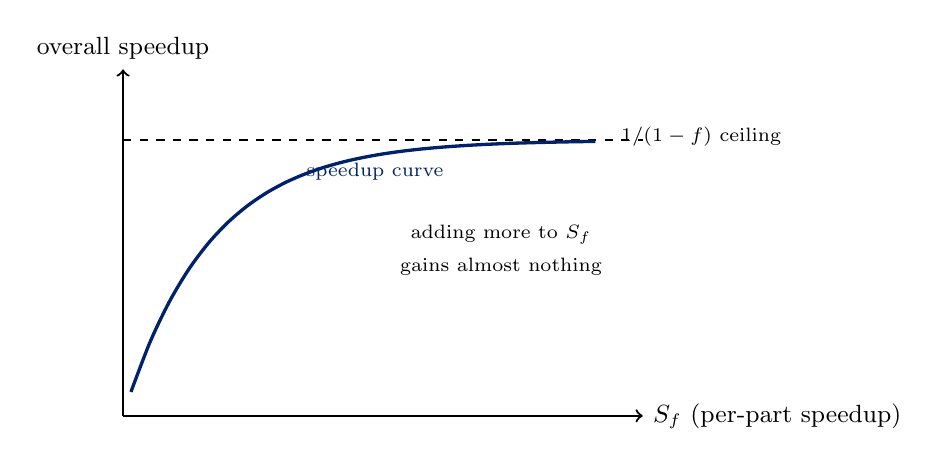
\begin{tikzpicture}[scale=1.0, transform shape,
        every node/.style={font=\small}]
      \draw[->, thick] (0,0) -- (6.6,0) node[right] {$S_f$ (per-part speedup)};
      \draw[->, thick] (0,0) -- (0,4.4) node[above] {overall speedup};
      \draw[thick, dashed] (0,3.5) -- (6.6,3.5);
      \node[font=\scriptsize, right] at (6.2,3.55) {$1/(1-f)$ ceiling};
      \draw[very thick, primary-blue] plot[domain=0.1:6.0, smooth]
        (\x, {3.5*(1 - exp(-\x/1.1))}) ;
      \node[font=\scriptsize, primary-blue] at (3.2,3.1) {speedup curve};
      \node[font=\scriptsize] at (4.8,2.3) {adding more to $S_f$};
      \node[font=\scriptsize] at (4.8,1.9) {gains almost nothing};
    \end{tikzpicture}
  \end{center}
  The curve saturates: even an \emph{infinite} speedup of the improved part
  cannot beat the unimproved fraction.
\end{frame}

\begin{frame}{Worked Example: Applying Amdahl's Law}
  \begin{block}{Setup}
    40\% of a program's time is spent on floating-point. A new FP unit makes
    that part 4$\times$ faster. Overall speedup?
  \end{block}
  \begin{exampleblock}{Plug in}
    $f = 0.4$, $S_f = 4$:
    \[
      \text{Speedup} = \frac{1}{(1-0.4) + 0.4/4} = \frac{1}{0.6 + 0.1} =
      \frac{1}{0.7} \approx 1.43\times.
    \]
  \end{exampleblock}
  \vspace{0.2cm}
  \muted{Even a 4$\times$ FP speedup on a 40\% fraction buys only 1.43$\times$
  overall --- the 60\% unimproved part dominates.}
\end{frame}

\begin{frame}{Worked Example: The Ceiling in Action}
  \begin{block}{Setup}
    Same program, 40\% FP. How much overall speedup is possible \emph{at
    best}, i.e.\ as the FP part becomes infinitely fast?
  \end{block}
  \begin{exampleblock}{Ceiling}
    \[
      \lim_{S_f\to\infty} \frac{1}{(1-f) + f/S_f} = \frac{1}{1-f} =
      \frac{1}{0.6} \approx 1.67\times.
    \]
  \end{exampleblock}
  \begin{alertblock}{Design implication}
    If you want a program to run 3$\times$ faster and FP is only 40\%, the FP
    unit is the \emph{wrong place to invest} --- even infinite FP speedup
    cannot reach 3$\times$. You must also speed up the other 60\%.
  \end{alertblock}
\end{frame}

\begin{frame}{Socratic Check: The Parallelism Twist}
  \begin{alertblock}{Question}
    Amdahl's Law is often quoted against parallel computing: ``even with
    infinite processors, the serial fraction limits speedup.'' Is that right,
    and what is the one assumption that makes it optimistic or pessimistic?
  \end{alertblock}
  \begin{itemize}
    \item Right: serial fraction $(1-f)$ caps speedup at $1/(1-f)$.
    \item The assumption: $f$ is \key{fixed}. If the problem \emph{grows}
      (larger $n$), the parallel fraction usually grows with it --- so larger
      problems extract more parallelism, softening the ceiling. Amdahl's Law
      is a statement about \emph{fixed-size} workloads.
  \end{itemize}
\end{frame}

\transitionslide{One equation, three components, and a law about limits. Now: put it all together.}

% =============================================================================
% ACT 5 --- SYNTHESIS
% =============================================================================
\section{Synthesis}

\begin{frame}{The Thread, Closed}
  \begin{block}{What we built today}
    \begin{itemize}
      \item \key{Time} is the only honest speed measure: $\text{time} =
        \text{IC} \times \text{CPI} \times T_c$.
      \item \key{IC} (architecture), \key{CPI} (organization), $f$
        (technology) --- three independent levers.
      \item \key{MIPS} misleads when instruction sets differ; time never does.
      \item \key{Amdahl's Law} tells you which lever is worth pulling --- and
        which is not.
    \end{itemize}
  \end{block}
  \begin{exampleblock}{The running comparison}
    Machine A (2 GHz, CPI 2) and Machine B (3 GHz, CPI 3) tied at 10 ms for a
    $10^7$-instruction program; improving B's CPI to 1.5 made it 2$\times$
    faster --- a CPI (organization) win, not a clock-rate win.
  \end{exampleblock}
\end{frame}

\begin{frame}{Bridge to Week 2}
  \begin{block}{What's still missing}
    The performance equation assumes we can \emph{count instructions and CPI}.
    But before the CPU can execute anything, the \key{data} it works on must be
    represented in bits --- and arithmetic must be implemented in hardware.
  \end{block}
  \begin{exampleblock}{Next week}
    \key{Number systems}: how integers are represented (two's complement) and
    how adders/subtractors implement arithmetic in hardware --- the ``what the
    bits mean'' layer that the instruction set operates on.
  \end{exampleblock}
\end{frame}

\begin{frame}{Summary}
  \begin{itemize}
    \item \key{Architecture} = the programmer's interface; \key{organization}
      = the hardware implementation. Same architecture, different
      organization, different speed.
    \item \key{Basic structure}: CPU (ALU + registers + control) connected to
      memory and I/O by buses.
    \item \key{Performance equation}: $\text{CPU time} = \text{IC} \times
      \text{CPI} / f$ --- three independent factors.
    \item \key{Measurement}: time (or throughput) on a representative
      benchmark; beware MIPS.
    \item \key{Amdahl's Law}: $\text{Speedup} = 1\big/[(1-f) + f/S_f]$ --- the
      unimproved fraction sets an unbreakable ceiling.
  \end{itemize}
\end{frame}

\begin{frame}{References}
  \footnotesize
  \bibliographystyle{plain}
  \bibliography{../../Bibliography_base}
\end{frame}

\end{document}
